\documentclass[letterpaper, 11 pt]{article}
\usepackage[utf8]{inputenc}
\usepackage[spanish, mexico]{babel}
\usepackage{amsmath}
\usepackage{caption}
\usepackage{enumitem}
\usepackage{amsfonts}
\usepackage{apacite}
\usepackage{diagbox}
\usepackage{graphics}
\usepackage{amssymb}
\usepackage{parskip}
\usepackage{multicol}
\setlength{\columnsep}{1cm}
\usepackage{appendix}
\usepackage{textcomp}
\usepackage{graphicx}
\setlength{\parskip}{7pt}
\usepackage{float}
\usepackage[left=1.7cm,right=1.7cm,top=2cm,bottom=2cm]{geometry}
\usepackage{textcomp}
\usepackage{listings}
%\usepackage[breaklinks=true]{hyperref}

\begin{document}


\setlength{\unitlength}{1cm}
\thispagestyle{empty}
\begin{picture}(18,4)
\put(0,0){
\includegraphics[scale=.15]{unam.png}}
\put(14,0){
\includegraphics[scale=.19]{fac.png}}
\end{picture}

\begin{center}
\vspace*{0.2in}
{\fontsize{21}{21}\selectfont Universidad Nacional Autónoma de México}\\
\vspace*{0.2in}
{\fontsize{18}{18}\selectfont Facultad de Ciencias}\\
\vspace*{0.2in}
\begin{large}
{\fontsize{14}{14}\selectfont Laboratorio de Electromagnetismo} \\
\end{large}
\vspace*{0.2in}
\vspace*{0.2in}
\begin{Large}
\textbf{Práctica 1} \\
\textbf{La inducción de cargas eléctricas \\ por medio del frotamiento.} \\
\end{Large}
\vspace{.7 cm}
Integrantes del equipo:\\
Alonso Barradas Luis Gustavo\\ 
Fragoso Alvarado Daniel\\ 
Rios Fematt Mildred Stephany\\ 
Robledo Ibarra Emiliano\\
\paragraph{}
\begin{figure}[H]
    \captionsetup{justification=centering,margin=2cm}
    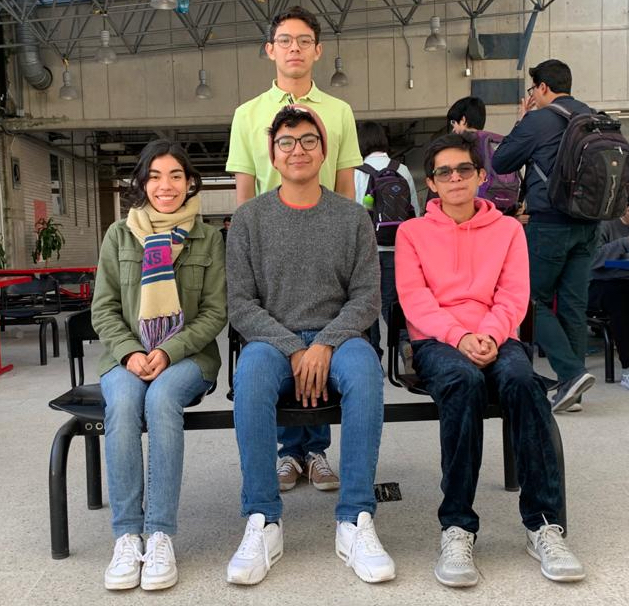
\includegraphics[scale=0.23]{uwu.jpg}
    \centering
    \caption{Equipo 3. Atrás: Luis Gustavo. \\ De izquierda a derecha:  Stephany Rios, Daniel Fragoso \\ y Emiliano Robledo.}
\end{figure}
\rule{80mm}{0.1mm}\\
\begin{large}
Profesora:  Fís. Maris Sofía Flores-Cruz.  \\
Ayudante: Miguel Ángel Amaya Reyes \\
Fecha de entrega: \today\\
\end{large}
\end{center}


\newpage

%%------------INICIO
\begin{multicols*}{2}

\section{Objetivos.}
Se plantean los siguientes objetivos a realizar:

\begin{enumerate}
    \item Comprobar la existencia de los dos tipos de carga usando un electroscopio e identificar sus efectos sobre él según la carga.
    \item Observar el comportamiento y algunas propiedades que se presentan entre los materiales cargados eléctricamente por medio del frotamiento, y  caracterizar ambos tipos de cargas.
\end{enumerate}

\section{Introducción.}

El entendimiento de las cargas eléctricas resultó fundamental para el desarrollo de los fenómenos electromagnéticos que formaron parte de las bases para el desarrollo electrónico que es uno de los hechos más relevantes de finales del siglo XX y lo que va del siglo XXI, sin embargo, su verdadera importancia radica en su necesidad para el entendimiento y descripción de fenómenos naturales, no solo de naturaleza atómica, sino también manifestaciones cotidianas (Resnick et al., 2002).

Los primeros en observar y estudiar las cargas eléctricas fueron los filósofos griegos; quienes descubrieron que al frotar una pieza de ámbar con un trozo de piel podía atraer algunos cuerpos ligeros; más tarde en 1600 el médico inglés William Gilbert \cite{Roller1953} observo que más materiales se comportaban como el ámbar; denominó a dichos materiales \textit{eléctricos} --de \textit{elektron}, la cual es la palabra griega para ámbar--, de dichas observaciones dedujo que como resultado del frotamiento los cuerpos adquieren una nueva propiedad que hoy llamamos \textit{electricidad}. Del mismo modo que caracterizamos la intensidad de la interacción gravitatoria mediante una masa gravitacional, podemos asignar una intensidad a esta fuerza mediante la \textit{carga eléctrica}.


En 1746 Benjamín Franklin, a la par que William Watson, llegaron a la conclusión, tras varios experimentos, de que únicamente existían dos cargas eléctricas; y para 1750 habían desarrollado una teoría de la electricidad basada en un experimento que mostró que un vidrio frotado recibió la misma carga eléctrica pero opuesta a la tela utilizada para frotarlo. Franklin identificó el término \textit{positivo} con electricidad vítrea y \textit{negativo} con electricidad resinosa \cite{Roller1953}. A este proceso de ganar o perder cargas eléctricas se le conoce como \textit{electrización} \cite{hewitt2007}; podemos encontrar tres formas de electrizar un cuerpo:

\begin{itemize}
    \item Frotamiento: al frotar repetidamente dos cuerpos eléctricamente neutros, ambos se cargan, uno con carga positiva y el otro con carga negativa.
    \item Contacto: ocurre cuando un cuerpo es puesto en contacto con otro cuya carga no es nula. Aquel cuerpo que presente un exceso relativo de carga la transferirá al otro.
    \item Inducción: cuando un cuerpo cargado se acerca a uno descargado sin llegar a tocarlo, las cargas en este último se reagrupan en dos regiones distintas del mismo.
\end{itemize}

Saber si un objeto fue electrizado, es decir si se encuentra eléctricamente cargado, se puede lograr mediante un electroscopio: el electroscopio es un aparato que permite demostrar la presencia de cargas eléctricas y comparar sus signos. Existen diferentes versiones, la más popular usa dos láminas o agujas metálicas delgadas unidas a un cuerpo conductor que a su vez se encuentra unido a una esfera metálica por la que se llevaran acabo las interacciones. Se suele insertar el conjunto en un bote de vidrio o un matraz para aislarlo del exterior. Cuando se acerca un objeto cargado eléctricamente parte de la carga pasa a las láminas,  que  al  tener  cargas  de  igual  signo  se  separan  por  repulsión  electrostática. Asimismo cuando el electroscopio tiene contacto con un objeto cargado, este quedará también cargado por contacto; a partir de este estado es posible conocer el signo de otras cargas según su comportamiento: en caso de que las laminillas se separen indica que tiene carga igual al instrumento de medición. Si las laminillas se cierran, el objeto tiene signo opuesto al electroscopio. \cite{electro}

\section{Desarrollo experimental.}
La realización de la práctica se dividió en dos partes; y se hizo uso de los siguientes materiales:

\begin{itemize}
    \item Varillas de diferentes materiales: vidrio, plástico, acrílico, PVC, latón, madera, nailon, aluminio, hierro.
    \item Diferentes tipos de tela: piel de conejo, poliéster, terciopelo,  manta, esponja, polar y raso.
    \item Electroscopio.
    \item Soporte universal.
    \item Varilla aislante con bola metálica.
    \item Hilo no conductor.
\end{itemize}

\section*{Parte A}

Consistió en la inducción de cargas eléctricas debida al frotamiento de una varilla con algún tipo de tela. Una vez frotadas las varillas con una tela se procedió a verificar si se le había inducido una carga a través de un electroscopio, por ello, para este primer desarrollo el dispositivo experimental fue únicamente el electroscopio (\textbf{Figura 3}), además, se requirió del uso de todas las telas y varillas. 


El primer experimento realizado --sección 1-- consistió en elegir una varilla y frotar un extremo de esta con un tipo de tela. Posteriormente, cuando se consideró adecuado, se acercó el extremo previamente cargado a la cabeza externa del electroscopio, evitando contacto entre ambos tal como se muestra en la \textbf{Figura 2}, con el fin de poder observar el efecto que la varilla frotada tenía sobre dicho aparato. Se repitió este procedimiento con todas las telas para cada varilla con el fin de conocer que combinaciones varilla-tela inducían una carga al ser frotadas.

\begin{figure}[H]
    \centering
    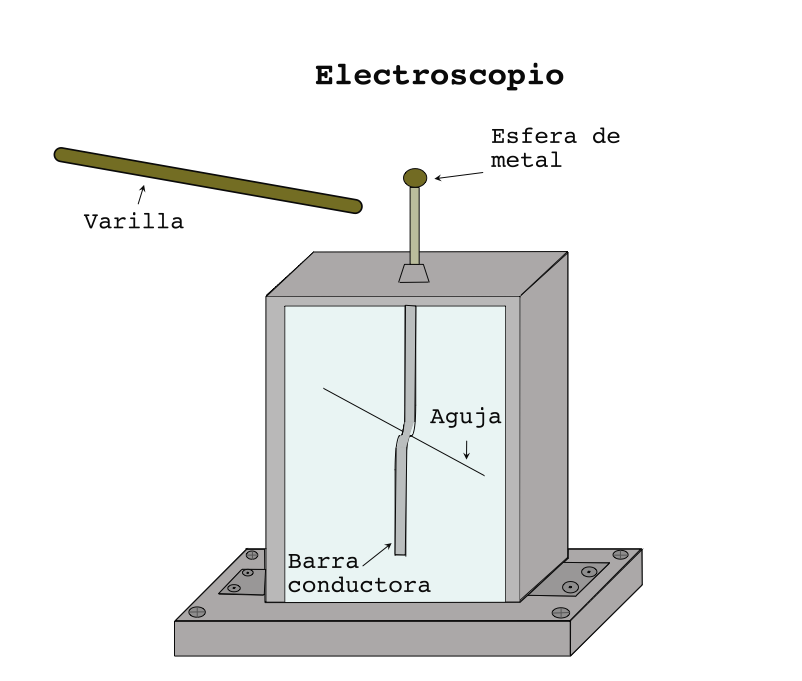
\includegraphics[scale=0.30]{el mamalon parte 1.png}
    \caption{Diagrama del electroscopio para la sección A}
\end{figure}

Posteriormente --sección 2-- se realizó una variación del primer experimento, es esta se llevó a cabo el contacto entre una varilla previamente cargada y la cabeza exterior del electroscopio, con el fin de observar las diferencias en el electroscopio en comparación con el solo acercamiento. Además, --sección 3-- se repitió el fenómeno anterior, es decir, tocar el electroscopio con una varilla cargada eléctricamente y una vez hecho esto, se acercó (sin tener contacto) a la cabeza del electroscopio otra varilla de un material distinto y cargada con una tela particular, se analizaron los efectos producidos de tal acercamiento. Finalmente, --sección 4-- se repitió el estado del electroscopio cuando una varilla cargada hace contacto con este, pero el fenómeno a analizar fue el contacto directo de la cabeza externa con un metal o la mano de un compañero una vez que electroscopio había sido cargado.

Es necesario mencionar que el electroscopio es un instrumento de medición construido para la comprobación de carga eléctrica, por lo que no se requirió la creación de un sistema especial para la obtención de mediciones en esta sección. En la \textbf{Figura 3} se muestra el arreglo experimental.
%%%%%%%%%%%%%%%%%%%%%%%%%%%%%%


%%ABRAN PASO AL MAMALON



\begin{figure}[H]
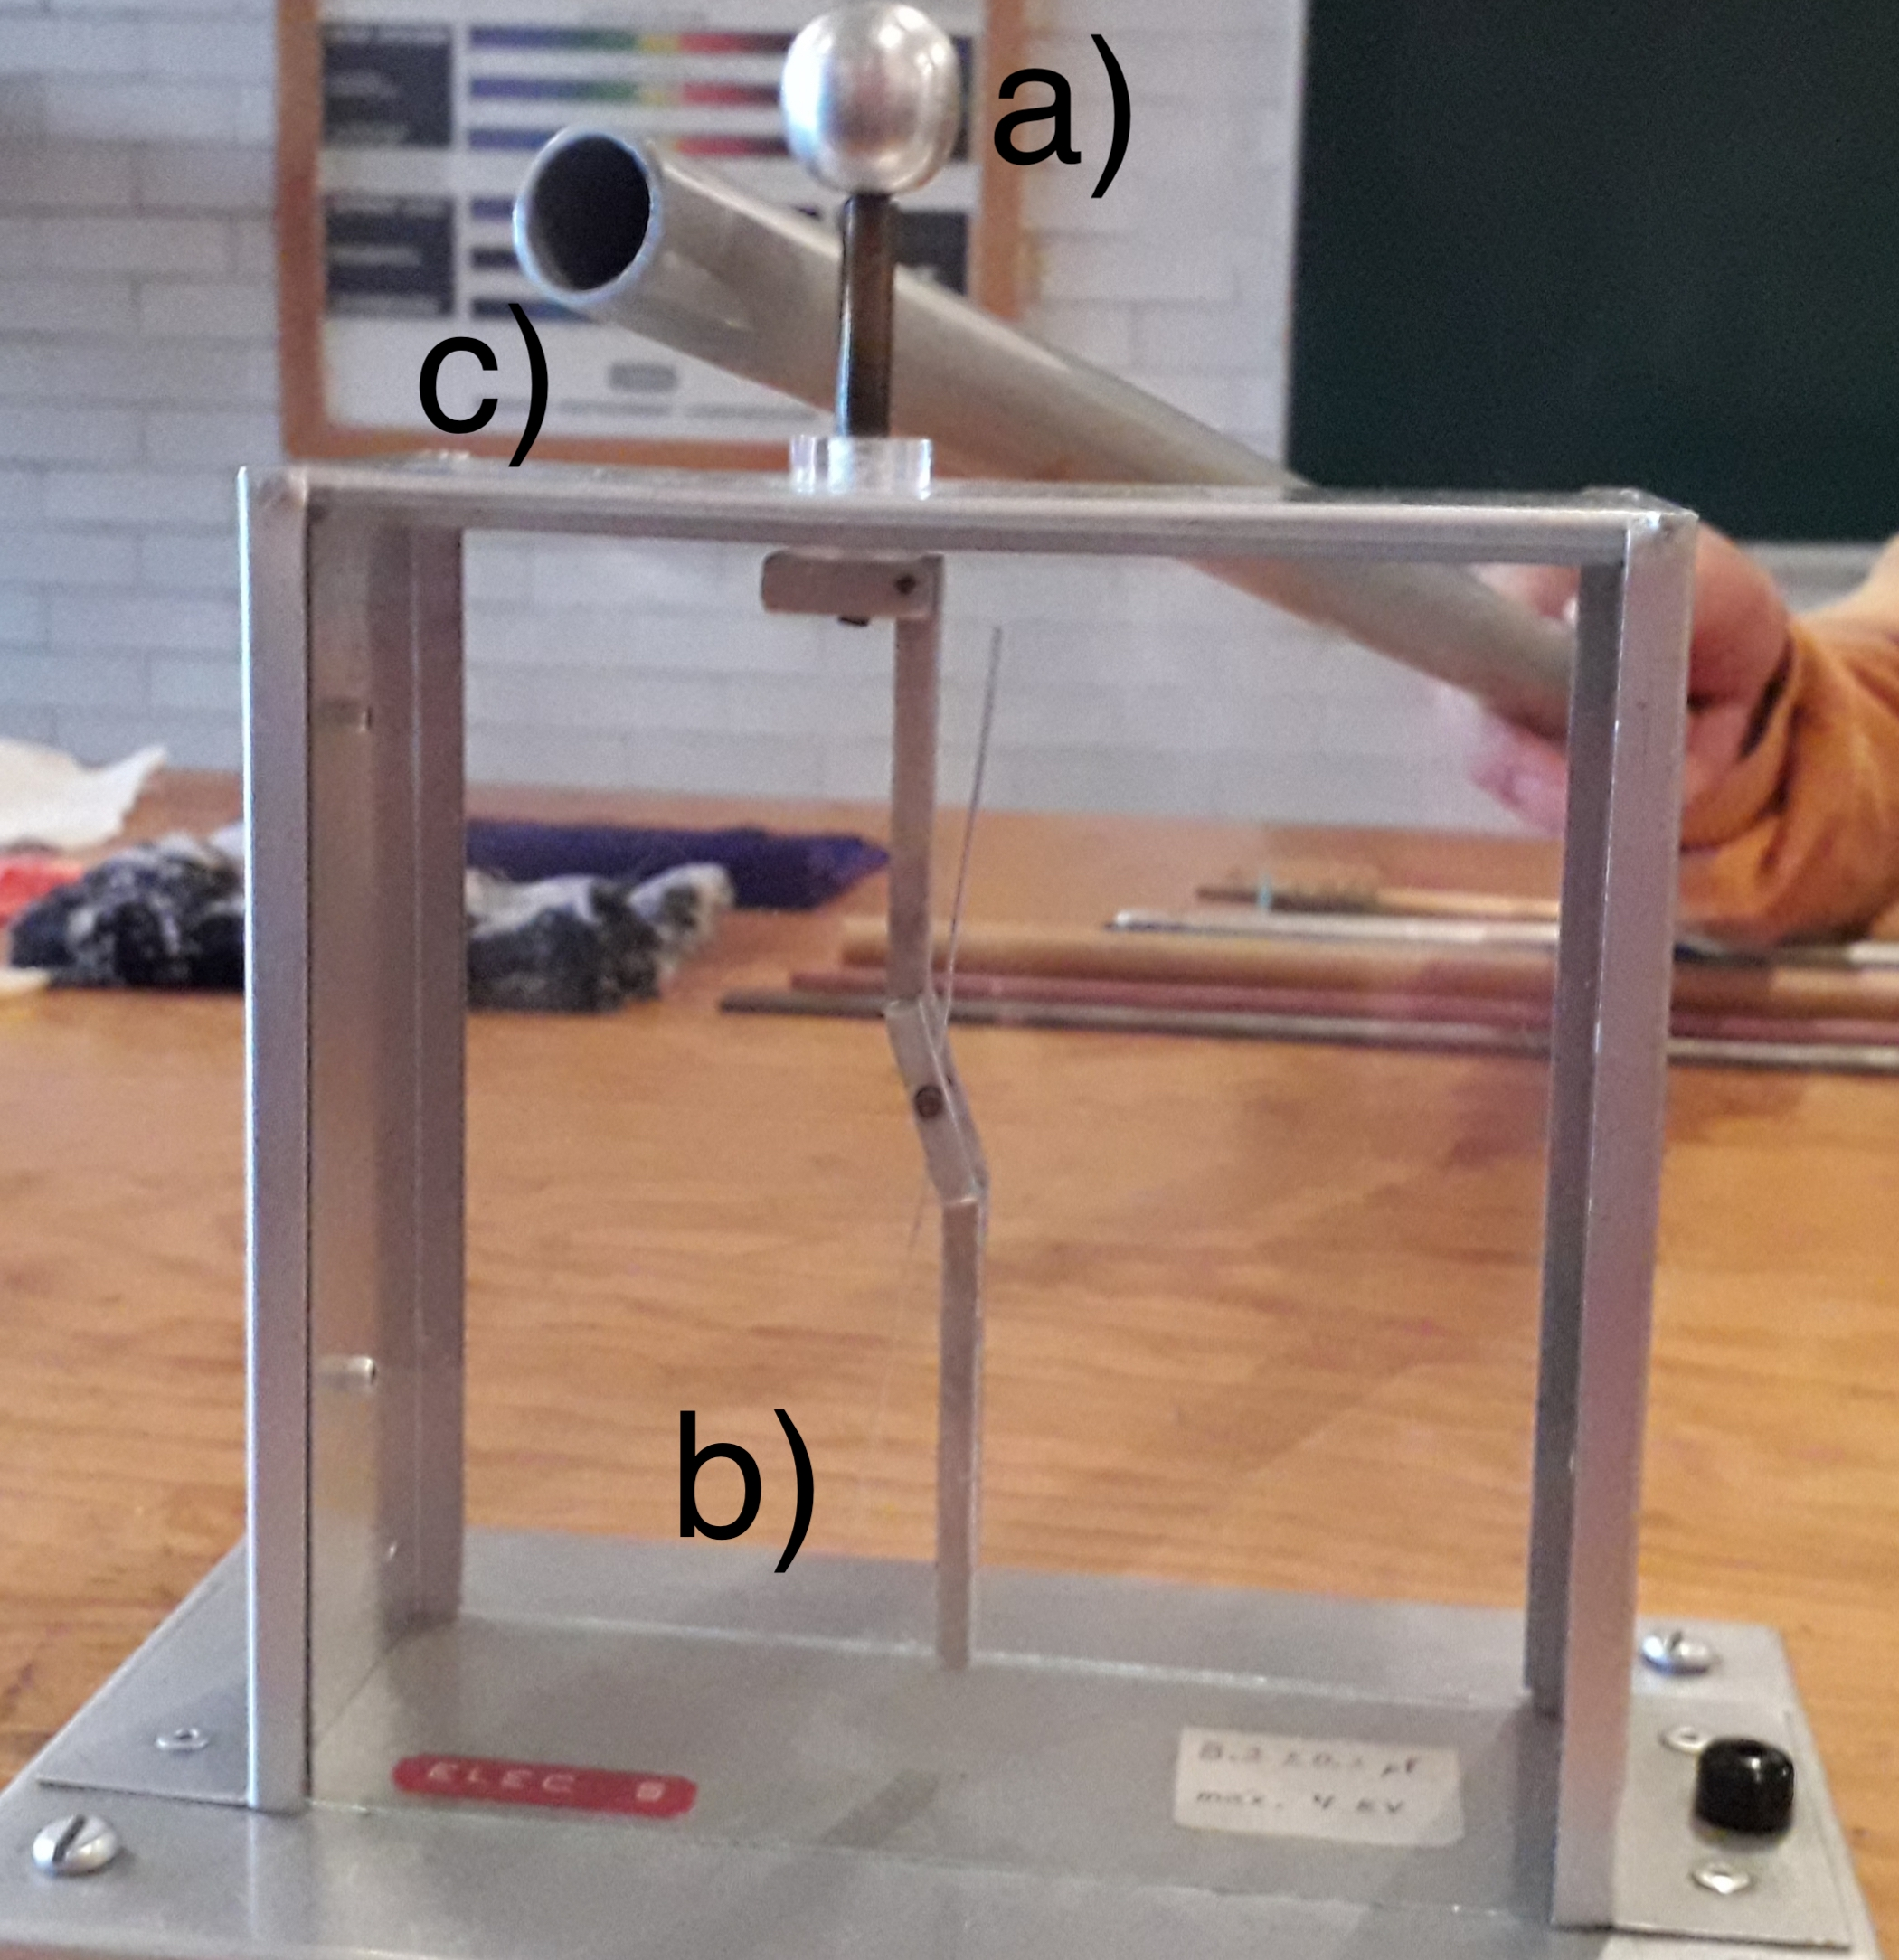
\includegraphics[scale=0.08]{electroscopio.jpg}
\centering
\small{\caption{Arreglo experimental sección A: a) Cabeza externa del electroscopio. b)  Aguja del electroscopio. c) Varilla eléctricamente cargada.}}
\end{figure}

\textbf{Parte B}

Por otro lado, la segunda parte de la práctica consistió en la observación del comportamiento de un tubo de PVC suspendido de un hilo no conductor bajo distintas interacciones de tipo electrostático; para dicho objetivo se requirió construir un sistema, como se muestra en la \textbf{Figura 4}, el cual utilizó un soporte universal que contaba con una varilla cilíndrica de nailon \footnote{El nailon, de acuerdo a UNITIKA (2019) dificulta la transmisión de cargas y su difusión, razón por la que la varilla del soporte universal fue elegida de dicho material.}, a esta varilla se le ajustó una nuez en la parte superior y gracias a dicha nuez se colocó una varilla más corta del mismo material de tal forma que resultasen perpendiculares entre sí, en el extremo de la segunda se amarraron dos tramos de hilos a los cuales se les realizó un nudo corredizo de forma que ambos hilos soportaran el tubo de PVC.
\begin{figure}[H]
    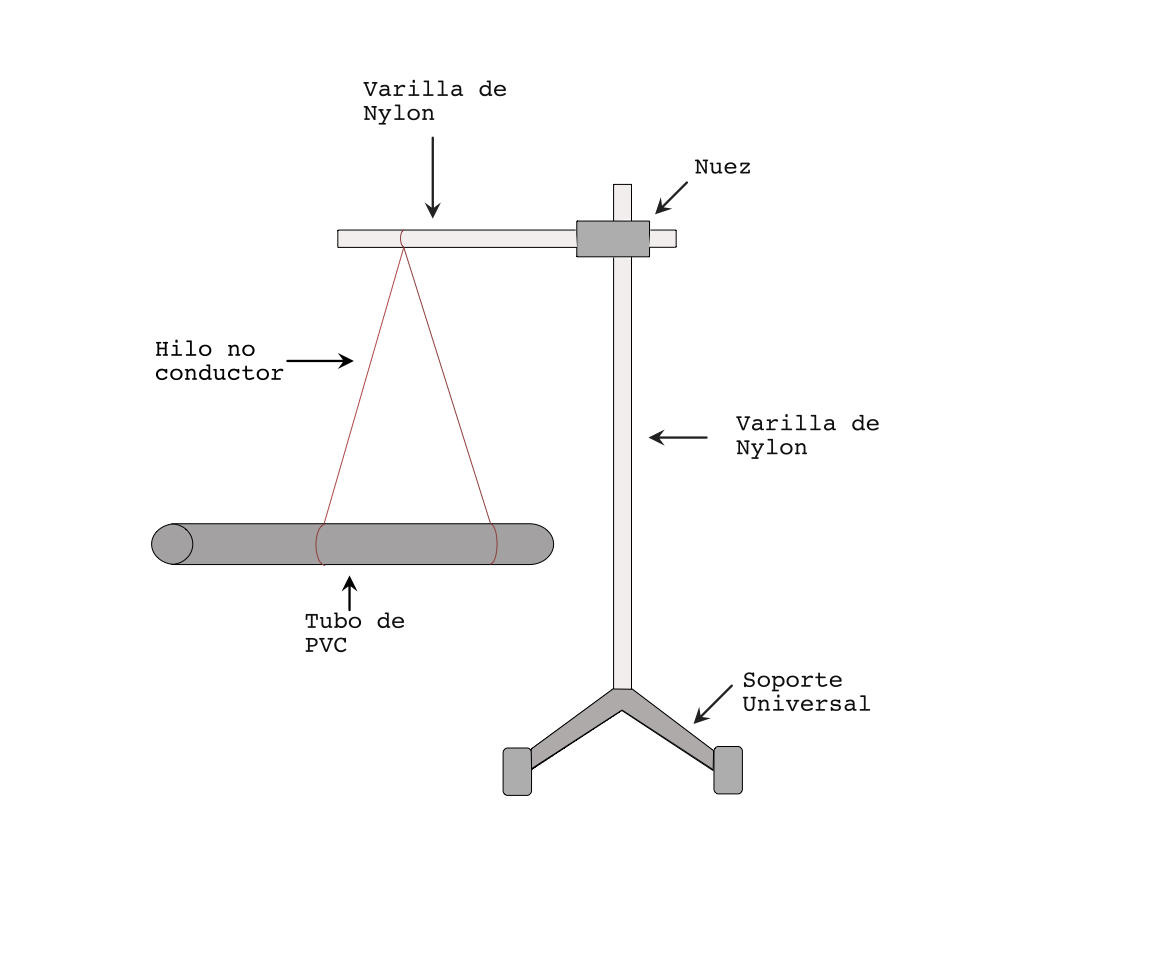
\includegraphics[scale=0.18]{mamalon2.png}
    \centering
    \caption{Diagrama del arreglo experimental sección B.}
\end{figure}
El tubo de PVC, una vez suspendido, fue frotado con esponja, pues la carga generada de esta interacción sería \textit{negativa} según se acordó como una referencia para la medición; una vez en reposo, al tubo --ahora cargado eléctricamente-- se le acercó una varilla de un material distinto previamente frotada con una tela --no necesariamente distinta-- como se aprecia en la \textbf{Figura 5}, según la reacción que se observó (y a partir del acuerdo de signo negativo que hicimos) pudimos atractiva o repulsiva en la varilla de PVC, fue posible identificar el signo de la carga que tenía cada varilla. Se comprobaron todas las telas para las varillas de plástico, vidrio, ebonita y latón.


%%%%%%%%%%%%
%ABRAN DOS PASOS PARA LOS SUPER MAMALONES

\begin{figure}[H]
    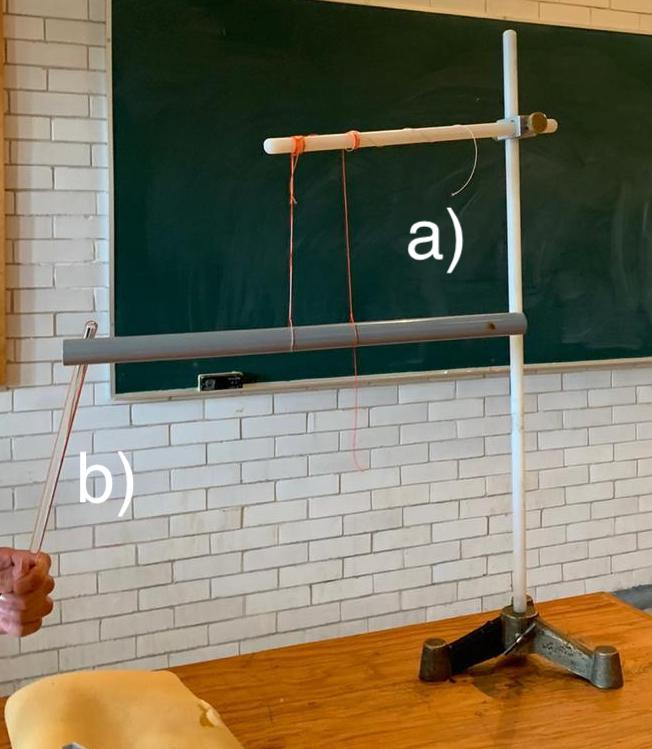
\includegraphics[scale=0.23]{pitotote.jpeg}
    \centering
    \caption{Aparato experimental: a) Sistema montado, tubo de PVC suspendido. b) Varilla eléctricamente cargada que se le acercó.}
\end{figure}
%%%%%%%%%%

\section{Resultados, análisis y discusión.}
A continuación se presentan los resultados de la primera sección de la parte A. Aquellas combinaciones varilla/tela que presentaron carga fueron marcados con una "$\times$", en general ninguna varilla de material metálico presentó carga, por lo que fueron excluidos de la siguiente tabla:

\begin{table}[H]
\begin{center}
\scalebox{0.8}{
\begin{tabular}{|c|c|c|c|c|c|}
\hline
\diagbox{Tela}{Varilla} & PVC & Plástico & Vidrio & Ebonita & Acrílico \\ \hline
Piel         & $\times$   & $\times$        & $\times$      & $\times$       & $\times$        \\ \hline
Manta        & -   & -        & $\times$      & -       & -        \\ \hline
Esponja      & $\times$   & -        & $\times$      & $\times$       & -        \\ \hline
Polar        & $\times$   & -        & -      & $\times$       & $\times$        \\ \hline
Raso         & $\times$   & -        & -      & $\times$       & $\times$        \\ \hline
Terciopelo   & $\times$   & -        & -      & $\times$       & -        \\ \hline
\end{tabular}}
  \caption{Combinaciones varilla-tela con las que se registró carga eléctrica.}
\end{center} 
\end{table}


Los materiales con los cuales se registró un cambio en el electroscopio en general son \textit{no metales} --aunque no todos los no metales sirven para este propósito como se puede observar en las mediciones--, además se pudo observar que todas las varillas no metálicas se cargan al frotarlos con la piel de conejo, asimismo, de los tres metales que se probaron ninguno de ellos se cargó de forma que se registrara cambio alguno en el electroscopio. Cabe aclarar que la aguja del electroscopio se comportó de manera distinta dependiendo del material y la tela con la cual se frotó ya que para materiales como el PVC (algunos sintéticos) la aguja lograba moverse hasta el otro extremo, es decir, giró 180º.

En primer lugar, observamos que aquí entra dos tipos de electrización: frotamiento e inducción. Ambos los comprobamos al acercar la varilla frotada y comprobar que la aguja del electroscopio se aleja de la base donde se encontraba. Observando los datos podemos notar que sólo no metales pudieron causar un efecto sobre el electroscopio, lo anterior se atribuye al hecho de que únicamente los materiales no conductores --dieléctricos-- son aquellos que no permiten que la carga se redistribuya a través de él, de esta manera al rozar el material con la tela  cada uno adquirirá carga debido a sus propiedades físicas, el resultado al separarlos es que uno habrá adquirido una carga positiva y otro una negativa; por otra parte sabemos que los metales conducen electricidad, gracias a esto la carga que se intenta inducir en ellos viaja a través de este y se distribuye en toda su extensión, incluso podríamos pensar que llega al portador de la varilla. En resumen, se observa un efecto local --ya que permanece en el lugar donde se frotó-- de inducción de carga en los puntos donde se frotó las varillas no metálicas, puesto que el electroscopio muestra la presencia de una carga pero en cuanto a las metálicas al acercarlas no se observó ninguna perturbación, esto debido a que las cargas eléctricas se distribuyeron del lugar donde se frotó.

%%%%%%%% B %%%%%%%%%%%%
En cuanto a la segunda sección se cargaron las varillas por frotamiento, aquellas con las cuales se observó que sí hubieron cambios en el electroscopio resultado de la anterior sección, y se observó que para todas ocurría un fenómeno similar, al encontrarse en contacto la varilla cargada y la cabeza del electroscopio, este último adquiría una posición fija alejada de la barra conductora; sin embargo, se observó que dependiendo de la combinación de los materiales varilla-tela era la amplitud de la separación. No todas las combinaciones afectaban de la misma manera al electroscopio, y de manera parecida a la sección anterior, para las combinaciones varilla-tela donde la aguja se elevaba más al acercarse al electroscopio, eran ahora estas combinaciones donde la posición tenía amplitudes más grandes en comparación con otras. Este comportamiento nos hace pensar en que ambos casos se encuentran relacionados y que no todos los cuerpos se cargan de manera igual con las mismas telas, sino que depende de la combinación del material y la tela que se frotan. Al frotar la varilla esta se electriza por frotamiento, el electroscopio se encuentra eléctricamente neutro ya que no ha recibido ningún estímulo y, al entrar en contacto con la varilla sufre el fenómeno de electrización por contacto, de esta forma el electroscopio recibe parte de la carga que se encontraba en la varilla, al separar ambos la carga que se pasó al electroscopio, como no puede disiparla y/o compartirla, queda remanente de forma que la aguja se repele de la base y mantiene una posición fija.

%%%%%%%%% OJO SI QUIERES QUE LO EXPLIQUE AHI TE VA
% Los materiales gozan de distintas afinidades electricas (cosa que mencioné en el anterior, por ende cada combinación carga de manera distinta a la varilla (ya sea positiva o negativamente) y esta diferencia hace que la carga o la cantidad de electrones que gana o pierde la varilla despues de frotar sea distinta despues de frotar cosa que se verá reflejada en la amplitud, al tener contacto el electroscopio se carga electricamente y sse carga la barra conductora y la aguja, como ambos se cargan de manera igual (mismo signo) se repelen


%%%%%%%% C %%%%%%%%%%%%
Los resultados de la tercera sección de la parte A fueron los siguientes, donde en negritas esta la combinación varilla-tela con la que se cargó el electroscopio:

\textbf{Plástico con piel de conejo:}
\setlist{nolistsep}
\begin{itemize}[noitemsep]
    \item La varilla que se acercó al electroscopio una vez cargado fue la de vidrio cargada con manta. Se percibió un alejamiento de la aguja de la estructura de apoyo, este cada vez mayor conforme la varilla de vidrio se acercaba. Lo que nos indica que la varilla cargada con manta tenia la misma carga que la del electroscopio.
\end{itemize}

\textbf{Ebonita con terciopelo:}
\setlist{nolistsep}
\begin{itemize}[noitemsep]
    \item  La varilla aproximada fue la de plástico frotada con piel de conejo. Se produjo como consecuencia un acercamiento de la aguja a la estructura de apoyo. Es decir que tenia carga con signo opuesto a la carga inducida por el frotamiento de la varilla de ebonita con terciopelo.

\end{itemize}

\textbf{Acrílico con piel de conejo:}
\setlist{nolistsep}
\begin{itemize}[noitemsep]
    \item Después de haber cargado el electroscopio con la varilla de acrílico frotada con piel de conejo, se aproximó la varilla de plástico cargada con piel de conejo. El producto de tal acercamiento fue un alejamiento de la aguja de la estructura de apoyo. Es decir que tenia carga con signo igual a la del electroscopio. 

\end{itemize}

\textbf{PVC con piel de conejo:}
\setlist{nolistsep}
\begin{itemize}[noitemsep]
    \item Al haber un encuentro con el tubo de PVC cargado con piel de conejo y la cabeza del electroscopio, la aguja mostró un levantamiento mayor a comparación de todos los demás materiales cargados.
    Al acercar la varilla de ebonita cargada con piel de conejo, se contempló un ligero movimiento de la aguja hacia la estructura de apoyo.
\end{itemize}

\textbf{Vidrio con esponja:}
\setlist{nolistsep}
\begin{itemize}[noitemsep]
    \item La varilla acercada fue la de plástico cargada con piel de conejo, produciendo un alejamiento de la aguja de la estructura de apoyo. Es decir tenia la misma carga eléctrica que la varilla de vidrio frotada con esponja.
\end{itemize}

Se ha de recalcar que durante esta parte del experimento únicamente se tomaron en cuenta a aquellas varillas que sí mostraron efectos de su frotamiento con una cierta tela. 

Como consecuencia de haber tocado el electroscopio con una varilla previamente cargada este instrumento adquirió parte de esta carga tal y como se vio en la segunda sección (ya que en este caso actúa la inducción por contacto), teniendo en cuenta este hecho, al acercar (sin contacto directo) una varilla distinta, a su vez cargada, la aguja del electroscopio presentaba un efecto de acercamiento o alejamiento a la base dependiendo de la combinación varilla-tela que se le aproximaba. Se observó que para algunas combinaciones la interacción producía un efecto constructivo --como un símil en las ondas-- pues incrementaba la separación, sin embargo, para el resto de las combinaciones la reacción era contraria, es decir que se reducía la separación entre la aguja y la estructura base del electroscopio. 

Se puede apreciar que en este fenómeno actúa una combinación de los dos anteriores: por una parte, como se observó, la varilla se carga gracias a la acción de frotarla con la tela y esta carga queda presente en el lugar donde dicha acción se llevó a cabo, posteriormente se carga el electroscopio por contacto directo y ahora se encuentra con una carga (independientemente de su signo) que hace que la aguja se aleje de la barra conductora, al acercarle la otra varilla se observa un efecto parecido al presenciado en la primera sección, sólo que ahora es posible la observación de dos posibles movimientos, uno donde la aguja pasa del estado fijo a una mayor elevación y el otro donde llega a una menor; de esto vemos que ninguno cumple ambos y por ende, conociendo que está interactuando con objetos cargados, podemos pensar que se están observando dos cargas distintas, la primera que al acercarla incrementa la separación de la aguja y la segunda que la decrece.


%%%%%%%% PARTE D %%%%%%%%%%%%
En la cuarta sección de la primera parte se observó que el contacto del electroscopio con una varilla frotada producía que la aguja de este se quedara en reposo alejada de la estructura del electroscopio, y al tocar con la mano o con la bola metálica se producía un efecto en el cual la aguja siempre regresaba al estado inicial donde la aguja se encontraba en contacto con la estructura del electroscopio, se probaron todas la varillas que producían un efecto al contacto pero con todas ocurrió lo mismo, al tener contacto regresaba la aguja a su estado inicial.

En general, cuando hay contacto entre un objeto cargado con otro que no lo esta, la carga tenderá a distribuirse entre ambos de tal forma que el cuerpo regrese a un estado neutro; por ello cuando nuestra mano entra en contacto con el electroscopio, la carga se distribuye por nuestro cuerpo, que a su vez busca la forma de deshacerse de dicha carga por medio de los diferentes objetos con los que interaccionamos. Lo mismo ocurriría para la esfera metálica, sin embargo, logramos observar que el efecto fue menor, es decir que aún cuando ambos —electroscopio y esfera— estuvieron en contacto el electroscopio no siempre regresaba a su estado inicial como era de esperarse; esto debió de darse por el tamaño de la esfera, que no tenia suficiente superficie en la cual distribuir la carga del electroscopio, por lo que no lograba “descargar” del todo el electroscopio.
%%%%%%%%%%%%%%%%%% SEGUNDA PARTE %%%%%%%%%%%%%%%%%%%

\subsection*{Parte B }

En la segunda parte de esta práctica, al acercarle otra varilla previamente frotada con otras telas, el PVC del sistema mostrado en la \textbf{Figura 5}, reaccionó de cierta forma con las cargas adquiridas por la segunda varilla, como se mencionó en la anterior sección existieron dos comportamientos: atractivo o de acercamiento (+) y repulsivo o de alejamiento (-). La siguiente tabla muestra los resultados obtenidos de las mediciones realizadas:

\begin{table}[H]
\begin{center}
     \resizebox{\columnwidth}{!}{%
    \begin{tabular}{|c|ccccc|} \hline
    \diagbox{Varilla}{Tela}  & Piel  & Polar & Terciopelo & Raso  & Esponja \\ \hline
    Plástico & -     & +     & +     & +     & - \\
    Vidrio & +     & +     & +     & +     & + \\
    Ebonita & -     & +     & +     & +     & + \\
    Latón & +     & +     & +     & +     & + \\ \hline
    \end{tabular}%
    }
    \caption{Signo de la carga en función del comportamiento del PVC.}
\end{center}    
\end{table}

La varilla de PVC al estar pendiendo y en reposo, respondía al acercarle otra varilla cargada, al hacer esto el sistema funcionaba como un péndulo de torsión, sin embargo cada varilla provocaba una amplitud distinta y no con todas las varillas resultó claro un comportamiento atractivo o repulsivo. Tal como se observó en el primer experimento --Parte A--, existen interacciones atractivas --cuando el tubo de PVC se acercaba a la varilla cargada--, y repulsivas --cuando el tubo se alejaba de la varilla cargada-- según el signo de su carga.

Además, los datos nos indican que un solo material puede cargarse eléctricamente con distintas magnitudes de cargas --según la amplitud del movimiento que presentaba el tubo de PVC-- e inclusive con cargas positivas como negativas, dependiendo de la forma en la que esta se adquirió y el material con el cual se llevó a cabo el proceso de frotamiento. % No se si agregar más

\section{Conclusiones.}
%%%%%%%%%%%%%%%%%%%% Primera parte
El uso del electroscopio fue fundamental para la realización de esta práctica, gracias a dicho instrumento fue que se pudo identificar si un objeto era poseedor de carga, y fue posible comparar entre aquellos que presentaban una mayor concentración de carga con aquellos en los que no se distinguía diferencia alguna antes de haber sido cargados. A pesar de que su uso fue necesario para el desarrollo del experimento, en ocasiones no se podía distinguir si el objeto no presentaba carga alguna o simplemente la sensibilidad del electroscopio no era lo suficientemente grande para poder percibirlo; esta duda se aclaró un poco más al realizar la segunda parte de la práctica, donde se utilizó el tubo de PVC para poder identificar como éste material cargado con esponja actuaba sobre otras varillas cargadas con diversas telas.

Entre los resultados que podemos destacar de esta primera parte de la práctica, es el hecho de que gracias al electroscopio fue posible observar y usar los tres tipos de electrización con el fin de observar los dos tipos de reacciones cuando al electroscopio cargado por contacto se le acerca una varilla que induce otra carga sobre este: una que aumentaba la amplitud y una que la reducía. Gracias a ambas reacciones distinguimos dos tipos de cargas, que aunado a la segunda parte de la práctica confirmaron los dos comportamientos registrados. %Algo así IDK 

%%%%%%%%%%%%%%%%%%%% Segunda parte

Durante el segundo experimento se encontró también,  que al acercar al tubo de PVC una cierta varilla cargada con una tela (ver \textbf{Figura 5}), solamente ocurrían dos fenómenos: atracción y repulsión. Sin embargo, no ocurrían ambos a la vez, dándonos a conocer que la varilla que acercamos en efecto poseía carga debido al frotamiento con la tela y esta se mantenía en el cuerpo a pesar de interactuar (no por contacto directo) con otra varilla. Como consecuencia de esta segunda parte no sólo se pudo percibir a aquellas varillas cargadas, sino que se logró distinguir qué carga poseían, esto último como producto del acercamiento de diferentes materiales cargados con diferentes telas.

El efecto observado en la segunda parte de la práctica es debido a una interacción eléctrica, gracias a que es posible descartar la interacción gravitatoria sabiendo de antemano que la magnitud de esta es muy pequeña; se dedujo que si el PVC se veía atraído por la varilla cargada entonces esta última debía tener carga del signo opuesto y si resultaba una repulsión entonces la varilla tendría carga del mismo signo, esta deducción se debe a tres factores: haber establecido una convención sobre el valor de la carga, conocer la existencia de la dualidad en valores de cargas eléctricas y conocer las interacciones entre ambas cargas eléctricas. 

Finalmente se observó que un material puede cargarse eléctricamente con distintas magnitudes de carga e inclusive con cargas tanto positivas como negativas, esto dependiendo la forma en la que ésta se adquirió y el material con el cual se llevó a cabo. Es posible verificar esto en los comportamientos que se observaron en la segunda parte: en como el plástico y la ebonita podían atraer o repeler al tubo de PVC dependiendo de la tela con la cual eran frotados. Por medio de los resultados obtenidos podemos concluir que no todos los objetos se cargan con la misma facilidad, además de que ésta propiedad depende de su composición así como del material con el cual es cargado, en este caso cargando las varillas por medio del frotamiento con diversas telas. Y de igual manera, al ser cargados estos no siempre poseerán la misma cantidad y signo de la  carga, sino que dependerá del material con el cual hubo contacto. 

En general, en el primer experimento logramos identificar las varillas que debido al frotamiento con cierta tela adquirían carga eléctrica, y posteriormente identificamos sus propiedades de repulsión y atracción cargando el electroscopio a la par de acercar una varilla previamente cargada; finalmente para observar mejor este efecto de repulsión-atracción, y lograr caracterizar a las cargas, se realizó un segundo experimento con el tubo suspendido de PVC; tras una convención en el signo de carga generado por el frotamiento del tubo de PVC y la esponja, se logró identificar el signo de carga que cada combinación varilla-tela generaba, logrando así de forma general el cumplimiento de los objetivos planteados al principio de la práctica.

\nocite{*}
\bibliographystyle{apacite}
\bibliography{mybib}


\end{multicols*}


\end{document}